\section{Semantica}
Prima di addentrarci nelle dinamiche del linguaggio appena
definito, dobbiamo definire la \textbf{memoria}. Nel nostro
caso lo facciamo tramite la funzione
\[ \sigma : \Var \to \N \]
che, data una variabile in input, restituisce il suo valore
in memoria (operazione di lettura). Noi però siamo interessati
anche a modificare la memoria, definiamo quindi l'operazione
di \textbf{aggiornamento} tramite la funzione, o meglio il
funzionale a tre argomenti
\[
	- [ - / - ] : (\Var \to \N) \times
	\N \times \Var \to (\Var \to \N)
\]
che è definita come
\[
	\sigma [n / x](y) = \begin{cases}
		n         & \text{se } y = x  \\
		\sigma(y) & \text{altrimenti}
	\end{cases}
\]
e cambia il valore della variabile $x$ con $n$. Quando
cercheremo di accedere nuovamente alla variabile $x$ in
memoria, la funzione $\sigma$ ci ritornerà il valore aggiornato.

La \textbf{semantica} di un'espressione aritmetica è data
dalla seguente funzione di \textbf{valutazione}, in cui andremo
a scrivere il suo argomento principale, l'espressione aritmetica,
tra le parentesi $[[$ e $]]$, cui viene giustapposto il secondo
argomento, cioè la memoria in cui l'espressione va valutata.
\[ \xi [[-]] - : E \times (\Var \to \N) \to \N \]
Proviamo a capire come questa funzione si comporta quando
prende in input espressioni aritmetiche.
\begin{align*}
	\xi [[n]] \sigma              & = n         \\
	\xi [[x]] \sigma              & = \sigma(x) \\
	\xi [[E_1 + E_2]] \sigma      &
	= \xi [[E_1]] \text{ più } [[E_2]] \sigma   \\
	\xi [[E_1 \times E_2]] \sigma &
	= \xi [[ E_1 ]] \text{ per } [[E_2]] \sigma \\
	\xi [[E_1 - E_2]] \sigma      &
	= \xi [[ E_1 ]] \text{ meno } [[E_2]] \sigma
\end{align*}
Per adesso limitiamoci a notare che se diamo alla funzione di
valutazione un numero $n$, qualunque sia la memoria, questa
ci restituirà il numero stesso.

Se invece gli passiamo una variabile, questa ci restituirà
il valore della variabile in memoria, si fa infatti uso della
funzione $\sigma$.

Se invece passiamo una qualche operazione aritmetica, questa
verrà valutata come la somma (oppure sottrazione o prodotto)
delle valutazioni degli operandi.

\begin{example}
	Proviamo a valutare l'espressione
	\[ x \times 2 - ((y - 7) + 1) \]
	nella memoria $\sigma$ tale che
	\[ \sigma (x) = 3 \quad \text{e} \quad \sigma(y) = 5 \]
	I passaggi per risolvere l'esercizio sono i seguenti
	\begin{align*}
		  & \xi [[ x \times 2 - ((y - 7) + 1) ]] \sigma \\
		= & \xi [[ x \times 2 ]] \sigma \text{ meno }
		\xi [[ (y - 7) + 1 ]] \sigma
	\end{align*}
	come possiamo notare, quando c'è un'ambiguità tra le
	precedenze supponiamo di sapere quale sia l'ordine
	corretto. In questo caso valutiamo "prima" il meno.
	\begin{align*}
		= & (\xi [[ x ]] \sigma \text{ per } 2) \text{ meno }
		\xi [[ (y - 7) + 1 ]] \sigma                          \\
		= & (\sigma(x) \text{ per } 2) \text{ meno }
		\xi [[ (y - 7) + 1 ]] \sigma                          \\
		= & (3 \text{ per } 2) \text{ meno }
		\xi [[ (y - 7) + 1 ]] \sigma
	\end{align*}
	ora abbiamo semplicemente preso il valore $3$ dalla memoria
	per sostituirlo a $x$.

	\begin{align*}
		= & 6 \text{ meno } (\xi [[y - 7]] \sigma
		\text{ più } 1)                                  \\
		= & 6 \text{ meno } ((\xi [[y]] \text{ meno } 7)
		\text{ più } 1)                                  \\
		= & 6 \text{ meno } ((\sigma(y) \text{ meno } 7)
		\text{ più } 1)
	\end{align*}
	Di seguito $5 - 7 = 0$ perché stiamo utilizzando il
	\emph{meno ridotto}, il quale ritorna $0$ quando il
	minuendo è maggiore o uguale del sottraendo.
	\begin{align*}
		= & 6 \text{ meno } ((5 \text{ meno } 7)
		\text{ più } 1)                          \\
		= & 6 \text{ meno } (0 \text{ più } 1)   \\
		= & 6 \text{ meno } 1 = 5
	\end{align*}
	Il calcolo per il resto è abbastanza banale.
\end{example}

Passiamo ora alla semantica delle operazioni booleane, che
non si inventano nulla di diverso rispetto alle espressioni
aritmetiche. Semplicemente la funzione di valutazione è
definita in modo da restituire valori booleani.
\[ \B[[-]] - : \B \times (\Var \to \N) \to \text{Bool} \]
Come prima andiamo a vedere cosa succede per vari input a
tale funzione di valutazione.
\begin{align*}
	\B [[t]] \sigma            & = tt                           \\
	\B [[f]] \sigma            & = ff                           \\
	\B [[E_1 < E_2]] \sigma    & =
	\xi [[E_1]] \sigma \text{ minore } \xi [[E_2]] \sigma       \\
	\B [[\lnot B]] \sigma      & = \text{ not } \B [[B]] \sigma \\
	\B [[B_1 \lor B_2]] \sigma & = \B [[B_1]] \sigma
	\text{ or } \B [[B_2]] \sigma
\end{align*}
Lo stile di definizione seguito fino ad ora prende il nome di
stile \textbf{denotazionale} e si propone di associare una
funzione a ciascun operatore.

Ci sono vari modi per definire una semantica, noi per il
momento andremo a definire la semantica tramite un approccio
\textbf{operazionale}, ossia guidato dalla sintassi.

Quello che andremo a fare è definire una sorta di macchina
astratta che procede per passi discreti, apportando modifiche
discrete alle sue configurazioni o stati, che possiamo
immaginare come coppie $(\text{comando}, \sigma)$.

Tale macchina, che definisce la semantica di un linguaggio
di programmazione, prende il nome di
\text{sistema di transizioni} ed è identificato dalla coppia.
\[ (\Gamma, \to) \]
dove $\Gamma$ è la classe delle \emph{configurazioni} (nel
nostro caso sono coppie $(C, \sigma)$) e
$\to \subseteq \Gamma \times \Gamma$ è una funzione detta
\textbf{di transizione}.

Tale coppia definisce come il nostro programma evolve in base
ai comandi che dobbiamo eseguire e a come questi modificano
la memoria.

In realtà noi seguiremo un approccio di tipo
\textbf{Structural Operational Semantics} (o
\emph{small steps}), in cui ciascuna transizione
\[ (c, \sigma) \to (c', \sigma') \]
rappresenta un singolo passo di computazione, ossia la macchina
ha attraversato lo stato $(c, \sigma)$ e \emph{transisce} nello
stato $(c', \sigma')$.

Possiamo allora fare considerazioni del tutto analoghe a quelle
fatte per la MdT, ossia possiamo dire che una computazione è
la chiusura riflessiva e transitiva della funzione di
transizione. Formalmente
\[ (c, \sigma) \to^* (c', \sigma') \]
In questo caso una computazione termina (o converge) se
\[ (c, \sigma) \to^* \sigma' \]
Quello che si vuole è che la relazione descritta precedentemente
come \emph{passo di computazione} soddisifi i seguenti assiomi
e regole di inferenza
\begin{center}
	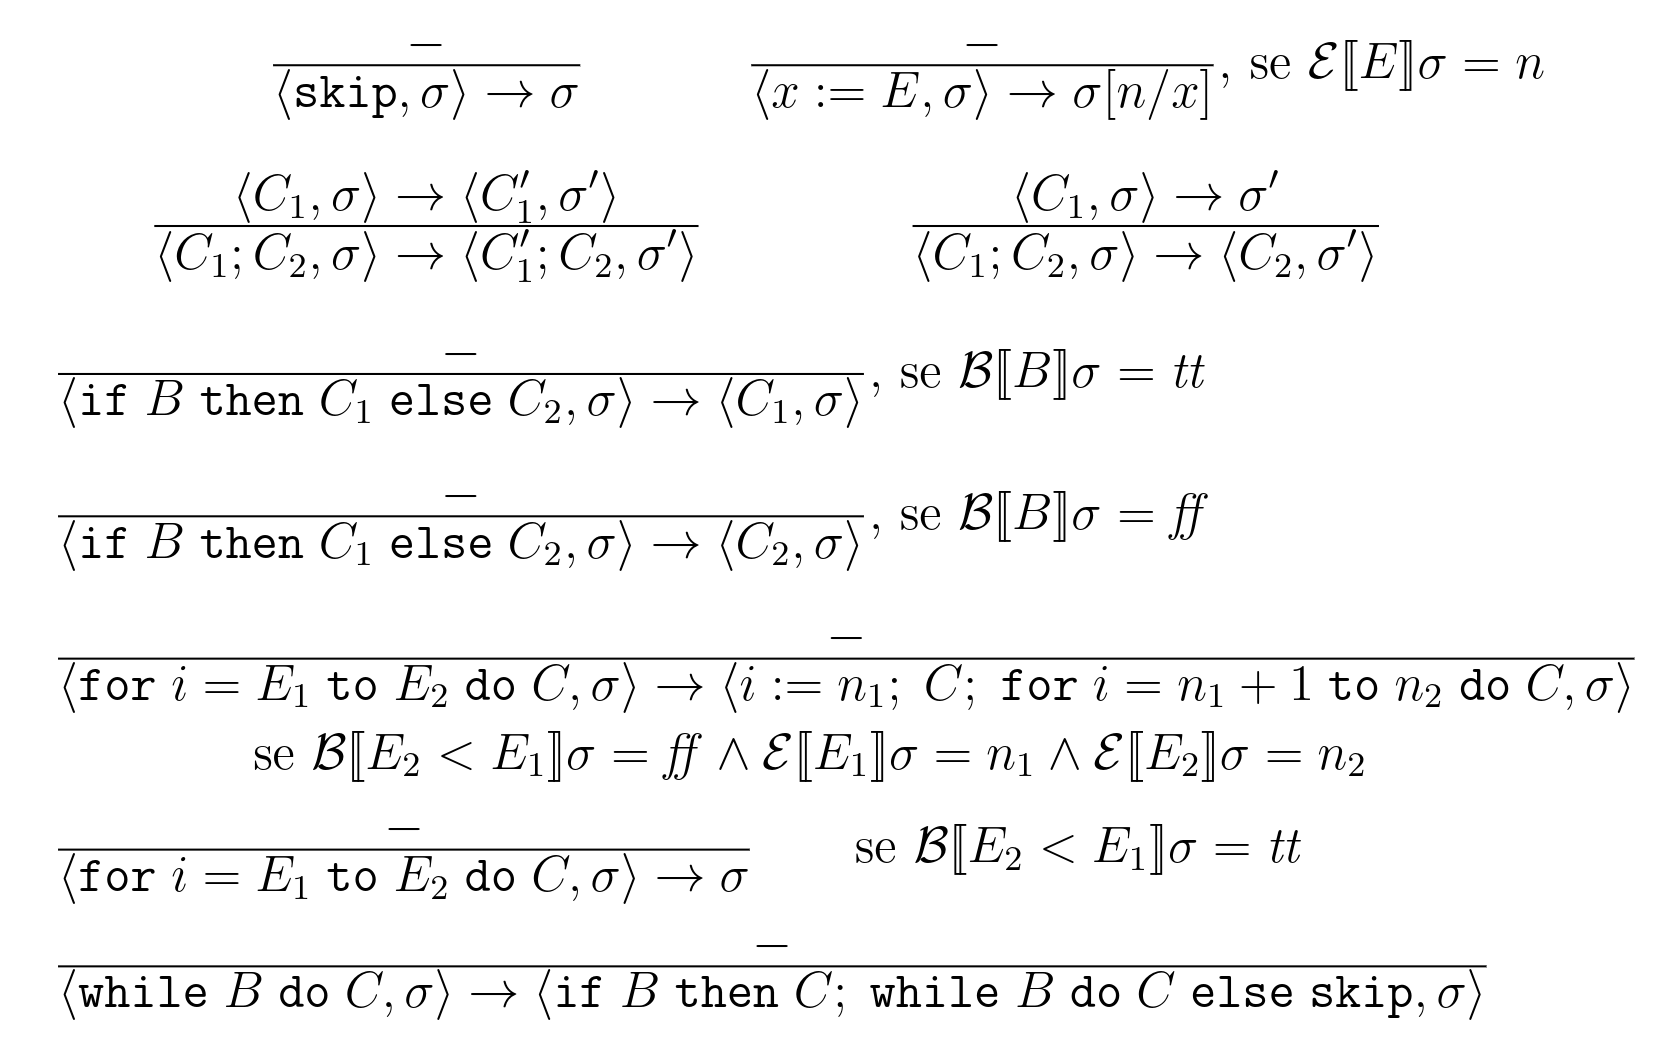
\includegraphics[scale=0.225]{images/assiomi.png}
\end{center}
Di particolare interesse è la regola di inferenza per
l'assegnamento, poiché chiarisce l'operazione di
\emph{aggiornamento} della memoria che avevamo lasciato in
sospeso.

Noi ci comportiamo come se la memoria fosse già inizializzata
per il nostro programma. Non ci sono vere e proprie operazioni
di scrittura della memoria. Ogni variabile esiste già in
essa e l'unica che cosa che ci è concesso fare è modificare il
suo valore.

Con la notazione $\sigma[n/x]$ intendiamo modificare il valore
della variabile $x$ presente in memoria con $n$. Stiamo in
realtà modificando la funzione che associa a $x$ un certo
valore (supponiamo $m$) con un altro valore ($n$).

La notazione che avevamo visto in precedenza per l'operazione
di aggiornamento significa che, se diamo $y$ in input a
$\sigma$ modificata, ossia $\sigma [n / x]$, se $y = x$,
allora stiamo in realtà cercando il valore di $x$ e dunque la
funzione ritorna $n$. Altrimenti stiamo cercando il valore di
$y$ presente in memoria e mai modificato dall'inizio
dell'esecuzione.

Per le altre regole teniamo a mente che, tutte quelle che
presentano una condizione a destra, si potrebbero scrivere
con la stessa condizione sopra.

In ogni caso per leggere le regole di inferenza seguiamo un
patter di questo tipo: se ci troviamo nello stato definito
descritto sotto la riga e a sinistra della freccia, si
transisce nello stato a destra della freccia se la condizione
è verificata.

\begin{example}
	Proviamo a dimostrare che il comando $C_1 ; C_2$ termina,
	tramite induzione.
	\begin{proof}
		Partiamo dalla regola di inferenza
		\[
			\frac{(C_1, \sigma) \to \sigma'}
			{(C_1 ; C_2, \sigma) \to (C_2 , \sigma')}
		\]
		e come ipotesi induttiva usiamo il fatto che se
		$C_1$ termina e $C_2$ termina, allora $C_1 ; C_2$
		termina. Se consideriamo la regola di inferenza
		\[
			\frac{(C_1, \sigma) \to (C_1', \sigma')}
			{(C_1 ; C_2, \sigma) \to (C_1' ; C_2 , \sigma')}
		\]
		il discorso è analogo con un passaggio in più. Se
		$C_1'$ termina ci ritroviamo al caso precedente e
		quindi anche $C_1 ; C_2$ termina.
	\end{proof}
\end{example}

\begin{example}
	Proviamo invece a dimostrare che il seguente programma
	\[ \text{while } tt \text{ do} \text{ skip}, \sigma \]
	non termina.
	\begin{proof}
		Per dimostrare che il programma non termina iniziamo
		a prendere la nostra configurazione di comandi e
		notiamo che corrisponde alla regola
		\[
			\frac{-}{(\text{while } B \text{ do } C, \sigma)
				\to (\text{if } B \text{ then } C;
				\text{ while } B \text{ do } C
				\text{ else skip}, \sigma )}
		\]
		che ci fa transire nello stato
		\[
			\text{if } tt \text{ then skip}, \sigma;
			\text{ while } tt \text{ do skip}, \sigma
			\text{ else skip}, \sigma
		\]
		a questo punto usiamo l'assioma dell'\verb|if| e
		otteniamo
		\[
			\text{skip}, \sigma ; \text{ while } tt
			\text{ do skip}, \sigma
		\]
		il primo comando è uno \verb|skip| e dunque ritorniamo
		al punto di partenza, ossia
		\[ \text{while } tt \text{ do} \text{ skip}, \sigma \]
		Ne concludiamo quindi che siamo entrati in un ciclo
		infinito.
	\end{proof}
\end{example}
